\chapter{Framework}

% **************************** Define Graphics Path **************************
\ifpdf
    \graphicspath{{Chapter3/Figs/Raster/}{Chapter3/Figs/PDF/}{Chapter3/Figs/}}
\else
    \graphicspath{{Chapter3/Figs/Vector/}{Chapter3/Figs/}}
\fi
In this chapter we present the basic framework of our vessel segmentation method. We start by setting up the various notation used throughout the chapter and give an overview about how the framework is applied.Next we discuss the two different models applied in the framework.This forms the core of this thesis and represents the major work done. At last we mention the various datasets utilized to test our models. In the next chapter we begin by running few experiments on the datasets to test the feasibility of models.\\
\section{Vessel segmentation Framework}
We start by defining the basic notations and methods. The input to our vessel segmentation framework is a training set composed of fundus images and their corresponding segmentation or label maps. The collection of fundus images is represented by $\bar{I} = (I^{(1)},I^{(2)}...., I^{(n)} )$  and their correspoding ground truth segmentation maps as $\bar{S} = (S^{(1)},S^{(2)}...., S^{(n)} )$. Each given image is of size M x N.
For simplicity, in the rest of the section a single image would be referred as I and S and the image I is a single channel image.\\

An image can be represented as a collection of overlapping patches computed around every pixel at center. A patch is of size $\sqrt{n}$ x $\sqrt{n}$ unless otherwise noted. We represent a patch centered at location (x ,y) as $p_{x,y}$, and patches for I and S can be represented as $Ip_{x,y}$ and $Sp_{x,y}$ respectively. For simplicity we can refer the pixels of patch as $\mathbb{P}_i$ for i =[1...n]. A patch is represented as a vector , obtained by concatenating the image patch values.\\

Now we can represent our datasets as 

%\begin{equation}
%	
%\bar{I} = \begin{pmatrix}
%	I^(1)\mathbb{P}_1 & I^(1)\mathbb{P}_2 & \cdots & I^(1)\mathbb{P}_n \\
%	I^(2)\mathbb{P}_1 & I^(2)\mathbb{P}_2 & \cdots & I^(2)\mathbb{P}_n \\
%	\vdots  & \vdots  & \ddots & \vdots  \\
%	I^(M)\mathbb{P}_1 & I^(M)\mathbb{P}_2 & \cdots & I^(M)\mathbb{P}_n \\
%	\vdots  & \vdots  & \ddots & \vdots  \\
%	I^(N)\mathbb{P}_1 & I^(N)\mathbb{P}_2 & \cdots & I^(N)\mathbb{P}_n 
%\end{pmatrix}
%
%\end{equation}
%
%
Fig~\ref{fig:fundus example} shows an example of fundus image on the left and the correspoding segmentation image on the right.\\

\begin{figure}
	\centering
	\begin{subfigure}[b]{0.45\textwidth}
		\centering
		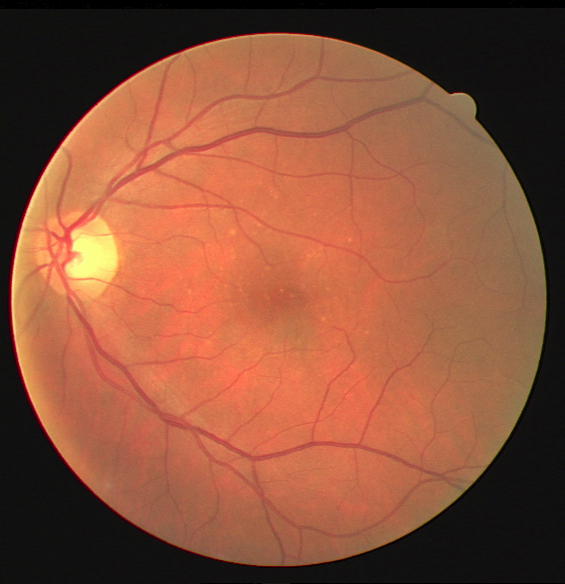
\includegraphics[width=\textwidth]{fundusimage}
		\caption{Fundus Image}
		\label{fig:fundusex}
	\end{subfigure}
	\hfill
	\begin{subfigure}[b]{0.45\textwidth}
		\centering
		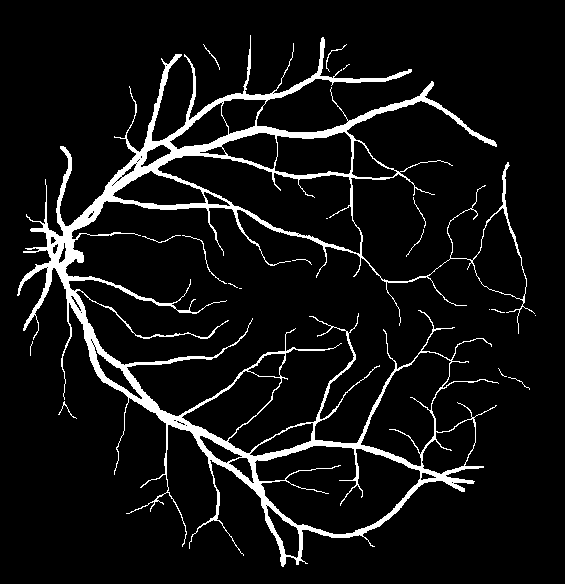
\includegraphics[width=\textwidth]{fundusimageseg}
		\caption{Segmented Vessels}
		\label{fig:fundusex seg}
	\end{subfigure}
	\caption{Fundus Image and its segmentation}
	\label{fig:fundus example}
\end{figure}

The aim of our thesis is to learn a function F which maps image I to its segmentation S, i.e, we want to learn a function to segment the vessel in a given fundus image. Inspired by works of [ref][ref] we approach the problem of prediction of segmentation maps in a  patch based framework. This means that to predict the segmentation map for an image I, we decompose the image into overlapping patches and predict the segmentation maps for individual patches. The image and the segmentation map after decompostion can be represented as in Equation [].

$$ F: I \rightarrow S $$

Here 'I' denotes the fundus image and 'S' its segmentation map.

At the test time, for a given image , we compute the patches and the mapping fucntion F is applied on all the test patches to obtain the segmentation.The output segmentation patches are combined by averaging ,thus resulting in an output segmented image.As the computed patches are overlapping, to each pixel several segmentation patches are added.More precisely, each pixel is composed of N pixel values.\\

In the next section we discuss how the mapping function F can be learnt. We present two models to predict the ground truth segmentation of a patch.


\section{Learning}
The major part of our work is to learn an effective mapping function F, to map the fundus image to its segmentation map.In our work, we learn a dictionary of representative image patches and a dictionary of segmentation patches. These dictionaries are then used to map the input image patch to its segmentation map. We explore two different methods to learn these dictionaries. Each image patch in the dictionary is denoted as an atom and our aim to find the best set of atoms so as to approximately infer closest segmentation. We notice that the these dictionaries resemble the local edge structure like junctions, stragight lines,crossover etc.

Before we explore the methods we list the common operation performed on out dataset.
 
\subsubsection{Preprocessing}
For our task we have explored some of the preprocessing steps including patch normalization, contrasts streching and local contrast normalization.
For all the experiments, we normalize each input patch by subtracting the patch mean and dividing by the standard deviation per patch. Also, all the input patches are vectorized before being fed to the predictor.

\subsubsection{Rotations}
To learn better image representations, we augmented the training set by adding the rotated pair of image and segmentation maps at an angle of 30,60,90,120 and 150 degrees. Adding rotations in general would help to learn better cases where the vessels might appear in different orientations.

%%%%%%%%%%%%%%%%%%%%%%%%%%%%%%%%%%%%%%%%%%%%%%%%%%%%%%%%%%
\section{Cluster Learning}
In our cluster learning framework, we learn an intermediate patch and segmentation maps. We then match our new patches to this dictionary and get the segmentation map from these images.
\subsection{Learning}

The training procedure for our method requires learning clusters within the input patches. Training is performed on the patches drawn from the input images $I_1$,$I_2$,...$I_n$ and corresponding segmentation images $S_1$,$S_2$,...$S_n$. 

From the training images, we compute a random subset of m patches of fixed size n x n and their corresponding annotation as computed from the segmentation images. This subset of patches is used to further learn a dictionary of patches and their annotations. Let us denote a patch as $x_i$ and its corresponding segmentation annotation patch as $y_i$. Then the new trainig set can be represented as:

$$
X = \{x_1,x_2,....,x_n\}
$$
$$
Y = \{y_1,y_2,....,y_n\}
$$
\\
We then find 'k' clusters within the patches in X usin K-Means clustering. Let the 'k' learnt cluster centers be represented as $C = \{c_1, c_2,..., c_k\} $ and the k clusters can be represented as $C_1,C_2,...,C_k$. A cluster with 'm' patches then can be represented as

$$
C_k = \{x^k_1,x^k_2,....,x^k_m\}
$$

Now, since we know the annotation $y_i$ for each training patch $x_i$, the image patches in each cluster can be repalced with their corresponding annotation patches to obtain the segmentation cluster as:
$$
SC_k = \{y^k_1,y^k_2,....,y^k_m\}
$$

We then find the representative point for the segmentation cluster by averaging all the patches belonging to it.
$$	
sc_k = \frac{1}{m}\sum\limits_{i=1}^{m} y^k_m
$$

Finally we create a dictionary mapping the cluster to their ground truth representatives as.
$$
D = \{ (C_k : gc_k) | k =1..m\}
$$

An example of dictionary learnt over image patches on DRIVE dataset is showin in figure[].

\subsection{Prediction}
At test time, the patches of an image are assigned to a cluster based on the learnt model.The desired annotation is then obtained by a lookup in the dictionary D.

\subsection{Algorithm}
The entire learning algorithm than can be summarized in following steps:
\begin{enumerate}
\item Extract a set of random Image-Segmentation patches of size m x m from the training images.

\item Train a K-Means clustering model on the input image patches and learn k clusters on the input.

\item Compute the ground truth patch for each cluster by averaging the ground truth annotations for each patch belonging to a cluster. 

\item Construct a dictionary of Cluster and annotations.
\end{enumerate}



\section{Dictionary Learning}

Our method is based on learning dictionary of patches from training data. In our methods we learn two dictionaries each for representing the image patches and their segmentations. The methods in a way is very similar to the above method where we associate a a learnt patch to its ground truth segmentation and use the dictionary for predicting new segmentations. The difference is in the way dictiontary of patches is learnt and the way in which a patch is matched to the dictionary. \\

Our proposed method is based on learning a spare dictionary of patches, of which a linear combination can be used to represent an image patch.
For each such image patches, denoted as dictionary atoms, we find a corresponding segmentation label patch.\\

For example, given an overcomplete dictionary of atoms D $\in$ $R^{m,k}$, with k columns as the learnt image atoms, we can reconstruct a given image patch x $\in$ $R^m$ as a linear combination of atoms in D. More formally, we learn a sparse code $\alpha$ over D to represent x as
$$ x \approx D \alpha $$  

\subsection{Learning}
The learning phase starts by extracting image and label patches from the training data. Let us represent our training set composed of random patches as,
$$
X = \{x_1,x_2,....,x_n\}
$$
$$
Y = \{y_1,y_2,....,y_n\}
$$
where X is composed of image patches and Y the corresponding label patches. Each image patch can be representated as a vector by concatenating each of the pixel values. So give, 'm' patches of size $\sqrt{n}$ x $\sqrt{n}$ , can be represented in form of matrices as 
X,Y $\in$ $R^{m,n}$. Each row in the matrice denotes a patch or image atom.

We learn an overcomplete dictionary  D of basis atoms from the image patches using the dictionary learning methods as described in[].
The aim is to learn a dictionary D with k atoms which can best represent $x_i$ using linear combination of a few atoms $d_k$ of the learnt dictionary.

In the next step we learn a sparse code $\alpha$ to represent our input X in terms of dictionary atoms.
$$
X = \alpha D
$$ 
Since we already know the ground truth annotation Y for X, we can infer that Y can be approximately represented as a linear combination of atoms from a dictionary of labels L, corresponding to D.\\

As the sparse code remains same for both the representations, we can compute the dictionary atoms from L by taking a weighted average of all the ground truth patches in Y, weighed by sparse codes for all the patches.\\

So we learn two dictionaries, D of image patches and L of the respective label patches for atoms in D.

\subsection{Prediction}
At the test time, given an image I, dense patches can be computed and the image can be represented as a matrix I $\in$ R, where each row represents a patch of size n x n. We then compute a sparse decomposition of I over dictionary D represented by a sparse code $\alpha$ such that:
$$
I = D \alpha
$$

We can then compute the ground truth segmentation S, for the image patches in I, as :
$$
S = L\alpha
$$
where $\alpha$ is the sparse code computed over dictionary D and L is the label dictionary previously computed during the learning phase.

%%%%%%%%%%%%%%%%%%%%%%%%%%%%%%%%%%%%%%%%%%%%%%%%%%%%%%%%%%
\section{Datasets}
For testing the performance of our algorithm , we train and test our system on the following publically available datasets. In this section we describe the characteristics of these datsets

\subsection{DRIVE}
The Digital Retinal Images for Vessel Extraction (DRIVE) dataset consists of 40 color retinal images randomly selected from diabetic retinopathy screening program for 400 diabetic patients.Each of these images in dataset are JPEG compressed and have a dimensions of 768 x 584 pixels captured at a resolution on bits per pixel. The images are captures with a 45degree field of view (FOV).
Of the 40 images in the datset, 7 show sign of diabetic retinopathy , while the remaining 33 do not consist of any pathology. Each image is provided with a corresponding mask delineating the FOV.\\

The dataset is divided is provided with divisions in terms of training and testing set, with each set consisting of 20 images. Each of the 40 images have been manually segmented by human observers trained by an experienced optamologist. For the training set, single ground truth segmentation of the vessels is provided. The test set is provided with two ground truth segmentations, of which the first one is used as gold standard and the other is used to compare the performance with an independent human observer.\\

\subsection{STARE}
The STARE dataset consists of 20 images with blood vessel segmentations, out of which 10 show signs of pathology. The images have been capture with a FOV of 35degrees at 8 bit per pixel resolution, with dimesnsions of each image as 605 x 700 pixels. The dataset consists of segmentation provided by two human observers. In our experiements, we consider the segmentations provided by the first observer as ground truth.\\

For the experiements, the dataset is randomly divided into training and test sets each consisting of 10images.

\subsection{HRF}
he High Resolution Fundus (HRF) image databse consists of 45 images of which 15 images come from healthy patients , 15 from patients with diabetic retinopathy and 15 of glacumatous patients. The images were captured with a FOV of 60degrees, at a high resolution of 24bits per pixel. The size of each image is 3504 x 2336 pixels and stored with JPEG compression. \\

Each image is provided a manual segmentation of vessesl as segmented by three independent human observers trained by experienced optahmologists.The dataset also provides a corresponging mask image of each image delineating the FOV.

\subsection{ARIA}
The ARIA dataset consists of three groups of images. One of the group consists of 92 images with age-related macular degeneration, the other with 59 images from diabetic patients and the last group with 61 images from a control group.\\

The images are captures with a 50degree FOV, stored in uncompressed TIFF format, with a resolution of 8bits oer pixel. Each image has dimensions of 768 x 576 pixels. The dataset provides with blood vessel segmentation images as manually segmented by experts and a corresponding mask delinating the FOV region.



\begin{table}
\caption{Summary of Datasets}
\centering
\label{table:datasets}
\begin{tabular}{c c c }
\toprule
{Datasets} & {FOV} &{\# of Images}  \\ \hline

DRIVE & 45 & 20+20 \\

STARE& 30 & 20  \\

HRF & 60 & 45  \\

ARIA & 50 & 212 \\

\bottomrule
\end{tabular}
\end{table}
